\documentclass{article}
\usepackage[polish]{babel}
\usepackage{minted}
\usepackage[letterpaper,top=2cm,bottom=2cm,left=3cm,right=3cm,marginparwidth=1.75cm]{geometry}
\usepackage{amsmath}
\usepackage{graphicx}
\usepackage[colorlinks=true, allcolors=blue]{hyperref}
\usepackage[T1]{fontenc}
\usepackage[table,xcdraw]{xcolor}
\usepackage{float}
\usepackage[figurename=Wykres]{caption}

\title{MOwNiT - Aproksymacja sredniokwadratowa wielomianowa}
\author{Jakub Frączek}

\begin{document}

\maketitle

\section{Funkcja dla której przeprowadzone zostało doświadczenie}

\begin{center}
\(f(x) = 10 * m + \frac{\mathrm{x}_{}^{2}}{k} - 10 * m * cos(k*x)\)
\end{center}

\noindent
gdzie:

\bigbreak

\(k = 1.5\)
\newline \indent
\(m = 3.0\)
\newline \indent
\(x \in [-4\pi, 4\pi]\)

\bigbreak

\noindent
Wykres funkcji:

\begin{figure}[H]
  \centering
  \begin{minipage}[b]{0.5\textwidth}
    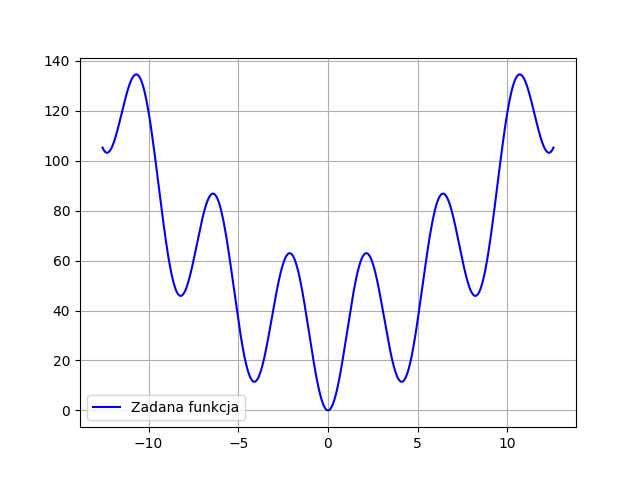
\includegraphics[width=\textwidth]{zadana_funkcja.png}
  \end{minipage}
\end{figure}

\section{Dane techniczne}

\subsection{Hardware}

Laptop z procesorem Intel Core i5-9300H 2.4GHz oraz 32 GB pamięci RAM.

\subsection{Software}

Wykorzystany został system Windows 11 x64 oraz język Python w wersji 3.11.8 wraz z bibliotekami:
\begin{itemize}
\item math
\item copy
\item matplotlib
\item numpy
\end{itemize}

\newpage

\section{Aproksymacja}

\noindent
Funkcja bazowe, czyli ciągi jednomianów \(\varphi _j(x) = x^i, j = 0, 1, ..., m\)

\noindent
Funkcja aproksymująca: \(f(x) = \sum_{j=0}^{m}a_j\varphi_j(x) = \sum_{j=0}^{m}a_jx^i\)

\noindent
F(x) - zadana na zbiorze dyskretnym \(\{x_i\}, i = 0, 1, ..., n\)

\noindent
Szukamy takich współczynników \(a_j\), że:

\[min!\sum_{i=0}^{n}w(x_i)[F(x_i) - f(x_i)]^2\]

\noindent
Układ normalny:

\[\sum_{i = 0}^{n}w(x_i)[F(x_i) - \sum_{j=0}^{m}a_jx_i^j]x_i^{k\longleftarrow \frac{\partial f}{\partial a_k}} = 0, k = 0, 1, ..., m\]

\[\sum_{i = 0}^{n}w(x_i)x_i^k\sum_{j=0}^{m}a_jx_i^j = \sum_{i=0}^{n}w(x_i)F(x_i)x_i^k, k =0,1,...,m\]

\[\sum_{j=0}^{m}(\sum_{i=0}^{n}w(x_i)x_i^{j+k}a_j = \sum_{i=0}^{n}w(x_i)F(x_i)x_i^k\]

\noindent
W postaci macierzowej:

\begin{gather*}
\begin{pmatrix}
\Sigma w_i & \Sigma w_ix_i & \Sigma w_ix_i^2 & \cdots & \Sigma w_ix_i^m \\
\Sigma w_ix_i & \Sigma w_ix_i^2 & \Sigma w_ix_i^3 & \cdots & \Sigma w_ix_i^{m+1} \\
\vdots & \vdots & \vdots & \ddots & \vdots \\
\Sigma w_ix_i^m & \Sigma w_ix_i^{m+1} & \Sigma w_ix_i^{m+2} & \cdots & \Sigma w_ix_i^{2m} 
\end{pmatrix} 
\begin{pmatrix}
a_0 \\
a_1 \\
\vdots \\
a_m 
\end{pmatrix}
= 
\begin{pmatrix}
\Sigma w_iF_i \\
\Sigma w_iF_ix_i \\
\vdots \\
\Sigma w_iF_ix_i^m 
\end{pmatrix}
\end{gather*}

\[G \cdot A=B\]

\section{Funckja wyliczająca aproksymację}

Po dyskusji na zajęciach i weryfikacji przeze mnie rozwiązania, okazało się, że aproksymacja jest wyliczana nie do końca prawidłowo. 
\bigbreak
\noindent
Funkcja przed poprawą wyglądała następująco:

\begin{minted}[bgcolor=lightgray]{Python}
def calculate_approx(xs, ys, m, w):
    
    G = np.zeros((m, m))
    B = np.zeros(m)
    
    for j in range(m):
        for k in range(m):
            
            G[j][k] = sum([w[i] * (xs[i] ** (j + k)) for i in range(len(xs))])
        
        B[j] = sum([w[i] * ys[i] * (xs[i] ** j) for i in range(len(xs))])
   
    A = np.linalg.solve(G, B) 
    
    return lambda x : sum([A[i] * (x ** i) for i in range(m)])
\end{minted}

\noindent
Natomiast poprawiona:

\begin{minted}[bgcolor=lightgray]{Python}
def calculate_approx(xs, ys, m, w):
    
    G = np.zeros((m + 1, m + 1))
    B = np.zeros(m + 1)
    
    for j in range(m + 1):
        for k in range(m + 1):
            
            G[j][k] = sum([w[i] * (xs[i] ** min(j + k, 2 * m + 1)) 
                                         for i in range(len(xs))])
        
        B[j] = sum([w[i] * ys[i] * (xs[i] ** j) for i in range(len(xs))])
   
    A = np.linalg.solve(G, B)
    
    return lambda x : sum([A[i] * (x ** i) for i in range(m + 1)])
\end{minted}

\noindent
Wniosek jest taki, że stopień wielomianu nie był wyliczany poprawnie i zmienna m wcześniej nie oznaczała stopnia wielomianu.

\section{Metody szacowania błędu przybliżenia funkcji}

Wszystkie błędy zostały policzone z dokładnością do 100 równoodległych punktów.

\subsection{Największa różnica wartości funkcji}

Największa różnica między wartością funkcji aproksymowanej, a funkcji aproksymującej:

\begin{center}
    \(\max_{x\in [a, b]} |F(x) - \mathrm{P}_{n}^{}(x)|\)
\end{center}

\subsection{Błąd średniokwadratowy}

Suma kwadratów różnic mięcy wartością funkcji aproksymowanej, a funkcji aproksymującej podzielona przez liczba punktów, w których wykonujemy porównanie:

\begin{center}
\(\frac{1}{N} * \sum_{i = 1}^{N}\mathrm{(F(\mathrm{x}_{i}^{}) - \mathrm{P}_{n}^{}(\mathrm{x}_{i}^{}))}_{}^{2}\)
\end{center}

\section{Analiza}

Podczas analizy funkcji aproksymującej,
węzły oraz stopnie wielomianów dobrałem zgodnie z poniższym twierdzeniem:

\begin{center}
Jeżeli \(x_1, x_2, ...,x_n\) są różne oraz m \(\le \) n, to G \(\neq \) 0
\end{center}

\noindent

Ponownie, po dyskusji na zajęciach ilość punktów wykorzystywanych przy liczdeniu błędów średniokwadratowego i maksymalnego oraz rysowaniu funkcji została zmieniona ze 100 na 1000.

\newpage

\section{Przebieg funkcji dla wybranej liczby węzłów}

\subsection{Dla 6 węzłów}

\noindent
Jak widać na poniższych wykresach (wykres 1, wykres 2, wykres 3, wykres 4), mimo małego błędu średniokwadratowego aproksymacja nie jest zbyt dobra.

\begin{figure}[H]
  \begin{minipage}[b]{0.49\textwidth}
    \begin{minipage}[b]{\textwidth}
      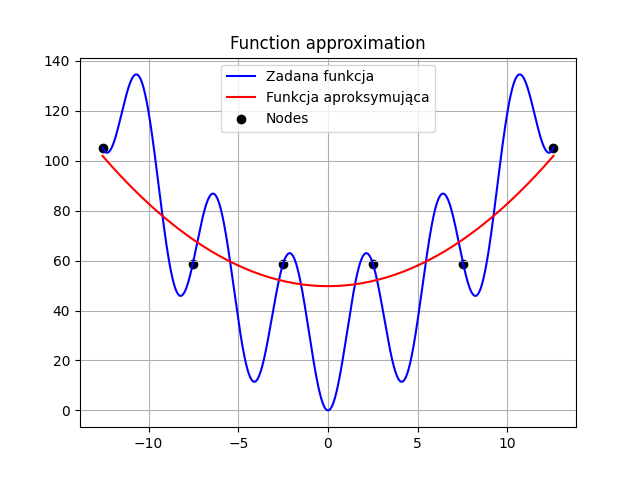
\includegraphics[width=\textwidth]{img01.png}
      \caption{Wielomian 3 stopnia}
    \end{minipage}
    \vspace*{\fill}
    \begin{minipage}[b]{\textwidth}
      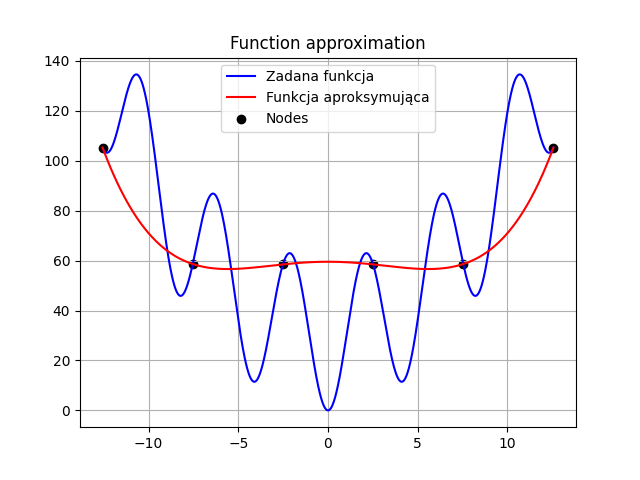
\includegraphics[width=\textwidth]{img02.png}
      \caption{Wielomian 4 stopnia}
    \end{minipage}
  \end{minipage}
  \hfill
  \begin{minipage}[b]{0.49\textwidth}
    \begin{minipage}[b]{\textwidth}
      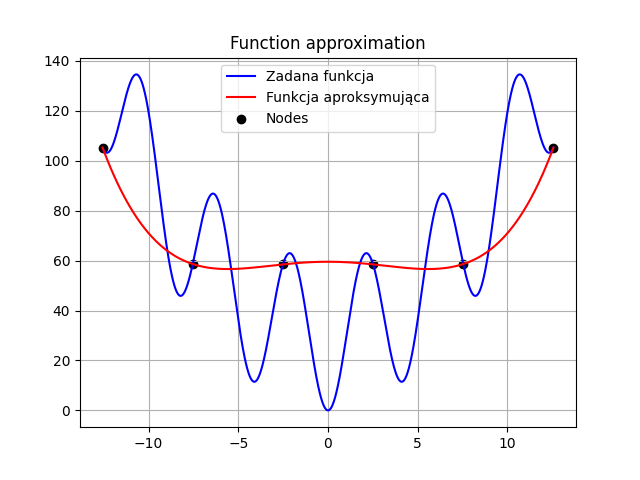
\includegraphics[width=\textwidth]{img03.png}
      \caption{Wielomian 5 stopnia}
    \end{minipage}
    \vspace*{\fill}
    \begin{minipage}[b]{\textwidth}
      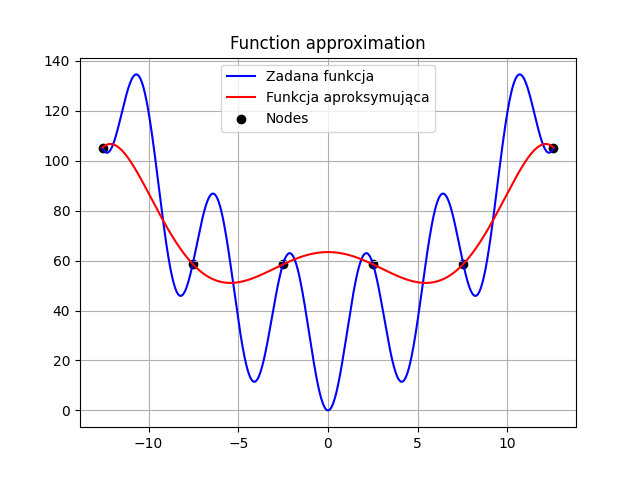
\includegraphics[width=\textwidth]{img04.png}
      \caption{Wielomian 6 stopnia}
    \end{minipage}
  \end{minipage}
\end{figure}

Poniżej, na wykresie 5 przedstawione zostały wartości błędów dla wszystkich możliwych stopni wielomianu.

\begin{figure}[H]
  \centering
  \begin{minipage}[b]{0.4\textwidth}
    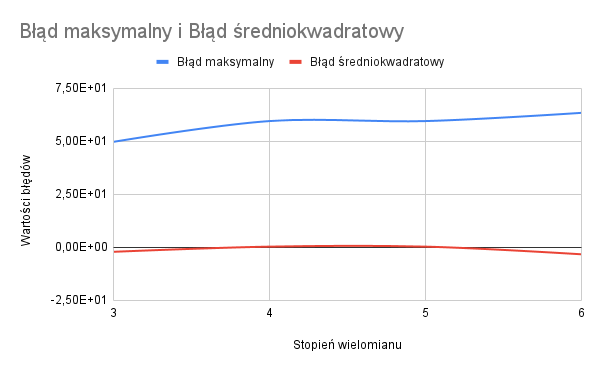
\includegraphics[width=\textwidth]{img05.png}
    \caption{Wartości błędów}
  \end{minipage}
\end{figure}

\newpage

\subsection{Dla 10 węzłów}

\noindent
Jak widać na poniższych wykresach (wykres 6, wykres 7, wykres 8, wykres 9), najlepsze przybliżenie otrzymujemy dla wielomianu stopnia 6, a dla wielomianóœ niższych i wyższych stopni przybliżenie jest coraz gorsze.

\begin{figure}[H]
  \begin{minipage}[b]{0.49\textwidth}
    \begin{minipage}[b]{\textwidth}
      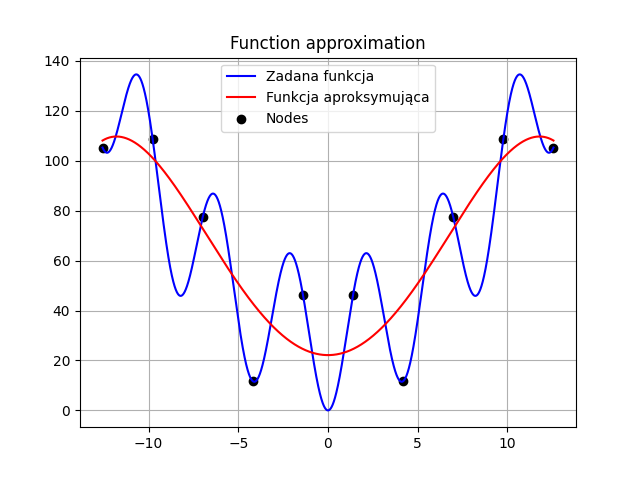
\includegraphics[width=\textwidth]{img06.png}
      \caption{Wielomian 5 stopnia}
    \end{minipage}
    \vspace*{\fill}
    \begin{minipage}[b]{\textwidth}
      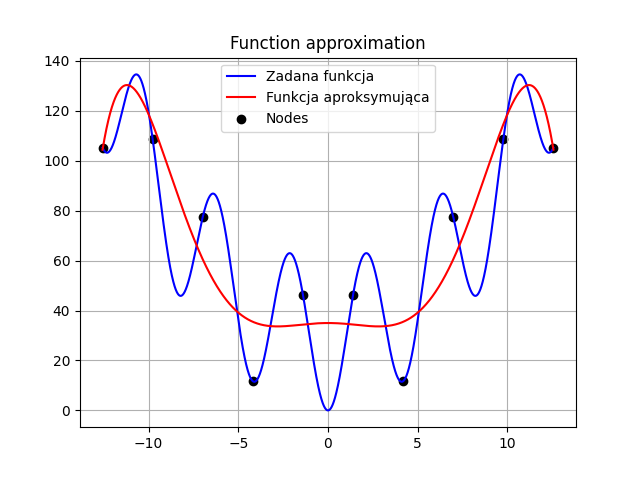
\includegraphics[width=\textwidth]{img07.png}
      \caption{Wielomian 6 stopnia}
    \end{minipage}
  \end{minipage}
  \hfill
  \begin{minipage}[b]{0.49\textwidth}
    \begin{minipage}[b]{\textwidth}
      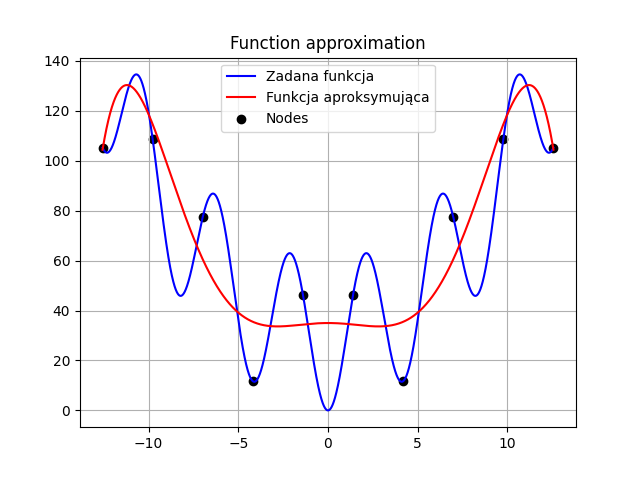
\includegraphics[width=\textwidth]{img08.png}
      \caption{Wielomian 7 stopnia}
    \end{minipage}
    \vspace*{\fill}
    \begin{minipage}[b]{\textwidth}
      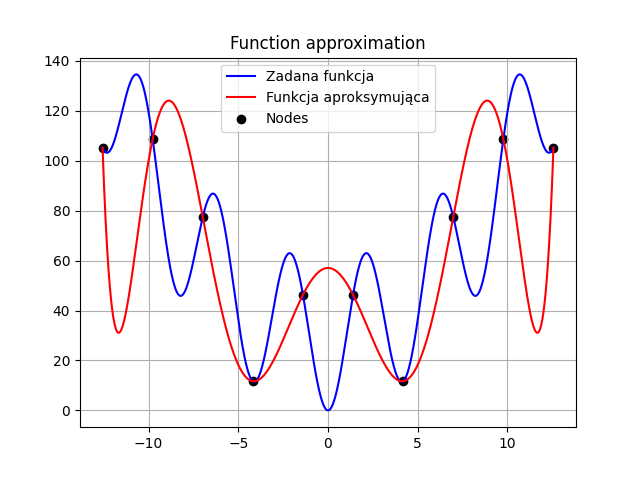
\includegraphics[width=\textwidth]{img09.png}
      \caption{Wielomian 8 stopnia}
    \end{minipage}
  \end{minipage}
\end{figure}

Poniżej, na wykresie 10 przedstawione zostały wartości błędów dla wszystkich możliwych stopni wielomianu.

\begin{figure}[H]
  \centering
  \begin{minipage}[b]{0.4\textwidth}
    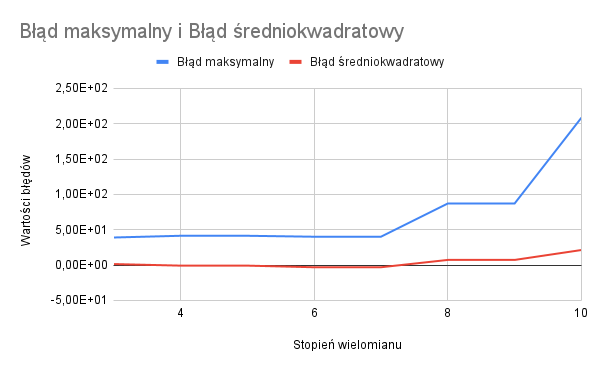
\includegraphics[width=\textwidth]{img10.png}
    \caption{Wartości błędów}
  \end{minipage}
\end{figure}

\newpage

\subsection{Dla 15 węzłów}

W tym przypadku przybliżenie, dalej nie jest dobre, najmniejsze błędy otrzymałem dla wielomianu 6-go stopnia, jedak, wielomian 8-go stopnia zdaje się lepiej przybliżać zadaną funkcję (wykres 11, wykres 12, wykres 13 i wykres 14).

\begin{figure}[H]
  \begin{minipage}[b]{0.49\textwidth}
    \begin{minipage}[b]{\textwidth}
      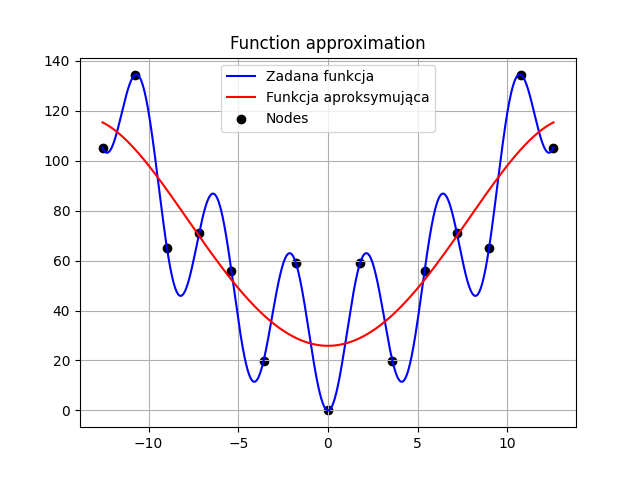
\includegraphics[width=\textwidth]{img11.png}
      \caption{Wielomian 5 stopnia}
    \end{minipage}
    \vspace*{\fill}
    \begin{minipage}[b]{\textwidth}
      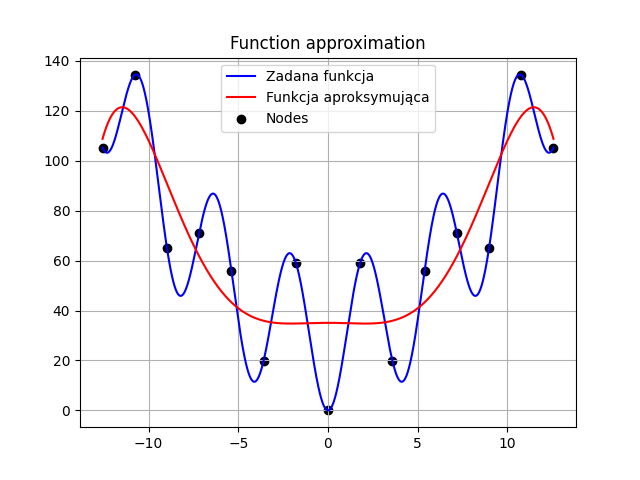
\includegraphics[width=\textwidth]{img12.png}
      \caption{Wielomian 6 stopnia}
    \end{minipage}
  \end{minipage}
  \hfill
  \begin{minipage}[b]{0.49\textwidth}
    \begin{minipage}[b]{\textwidth}
      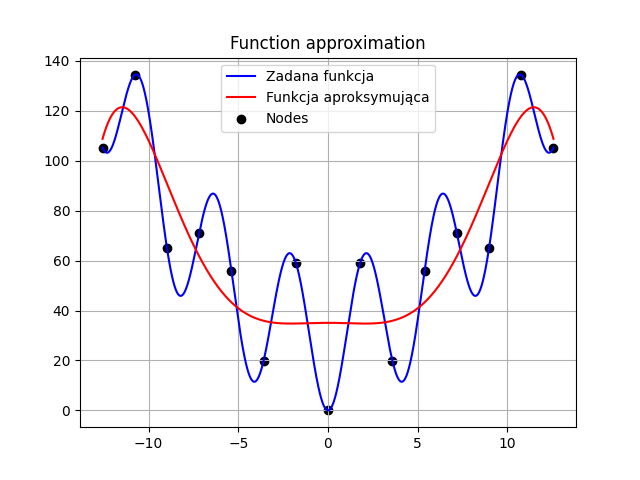
\includegraphics[width=\textwidth]{img13.png}
      \caption{Wielomian 7 stopnia}
    \end{minipage}
    \vspace*{\fill}
    \begin{minipage}[b]{\textwidth}
      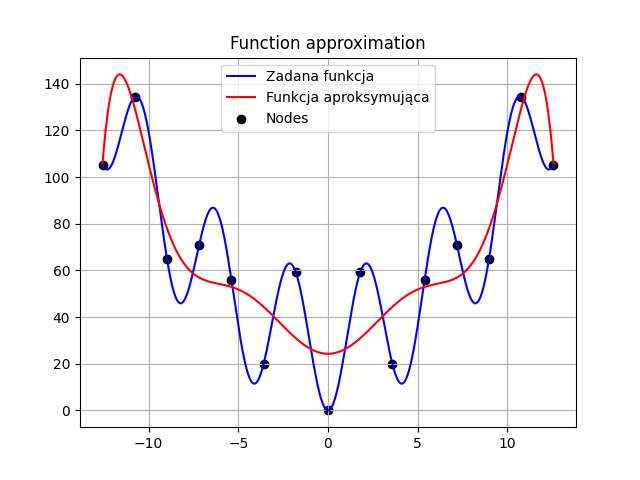
\includegraphics[width=\textwidth]{img14.png}
      \caption{Wielomian 8 stopnia}
    \end{minipage}
  \end{minipage}
\end{figure}

Poniżej, na wykresie 15 przedstawione zostały wartości błędów dla wszystkich możliwych stopni wielomianu.

\begin{figure}[H]
  \centering
  \begin{minipage}[b]{0.4\textwidth}
    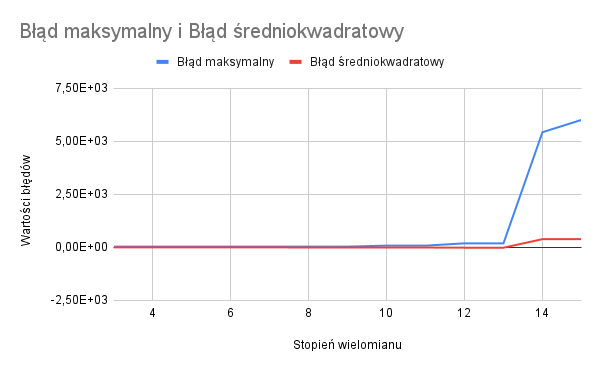
\includegraphics[width=\textwidth]{img15.png}
    \caption{Wartości błędów}
  \end{minipage}
\end{figure}

\newpage

\subsection{Dla 20 węzłów}

Jak widać na poniższych wykresach (wykres 16, wykres 17, wykres 18 i wykres 19), przybliżenie jest nieco bardziej dokładne, niż poprzednio. Najlepsze przybliżenie otrzymałem dla wielomianu 10-go stopnia, potem mimo, że w środku przedziału dopasowanie jest jeszcze lepsze, to na końcach znacznie zaczyna odbiegać od zadanej funkcji.

\begin{figure}[H]
  \begin{minipage}[b]{0.49\textwidth}
    \begin{minipage}[b]{\textwidth}
      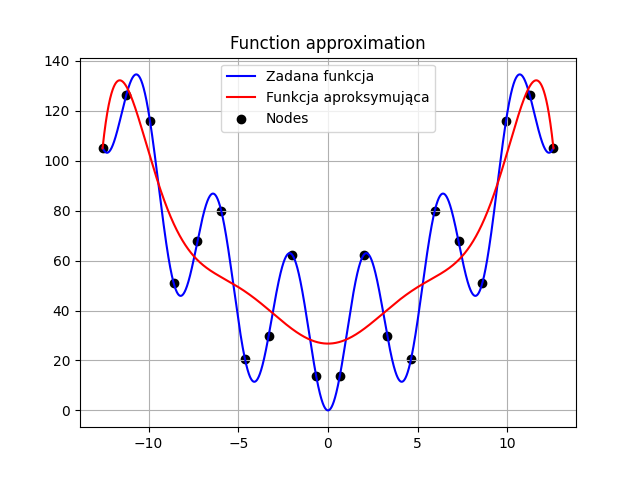
\includegraphics[width=\textwidth]{img16.png}
      \caption{Wielomian 9 stopnia}
    \end{minipage}
    \vspace*{\fill}
    \begin{minipage}[b]{\textwidth}
      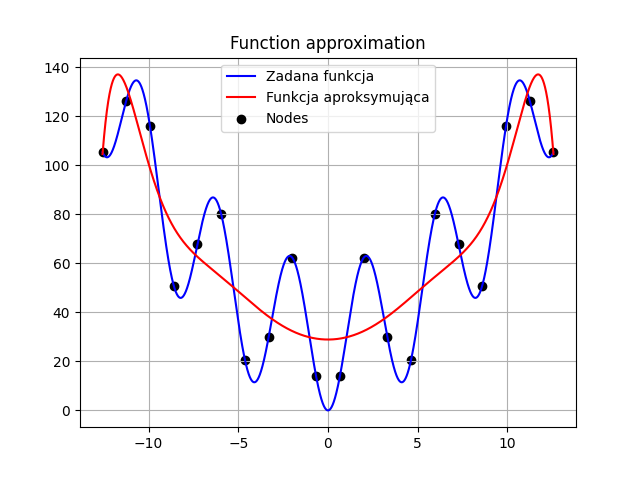
\includegraphics[width=\textwidth]{img17.png}
      \caption{Wielomian 10 stopnia}
    \end{minipage}
  \end{minipage}
  \hfill
  \begin{minipage}[b]{0.49\textwidth}
    \begin{minipage}[b]{\textwidth}
      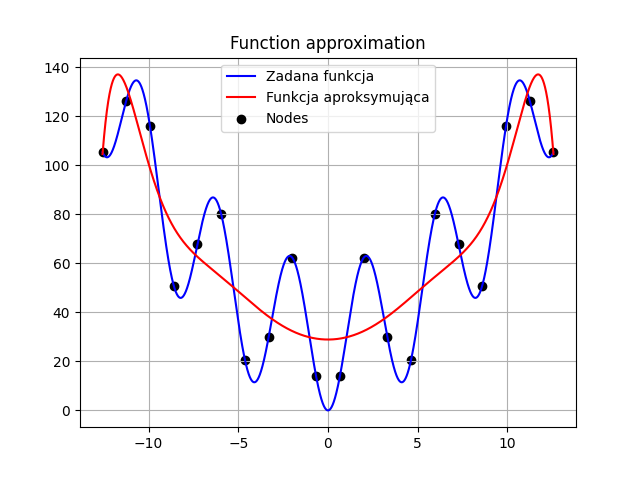
\includegraphics[width=\textwidth]{img18.png}
      \caption{Wielomian 11 stopnia}
    \end{minipage}
    \vspace*{\fill}
    \begin{minipage}[b]{\textwidth}
      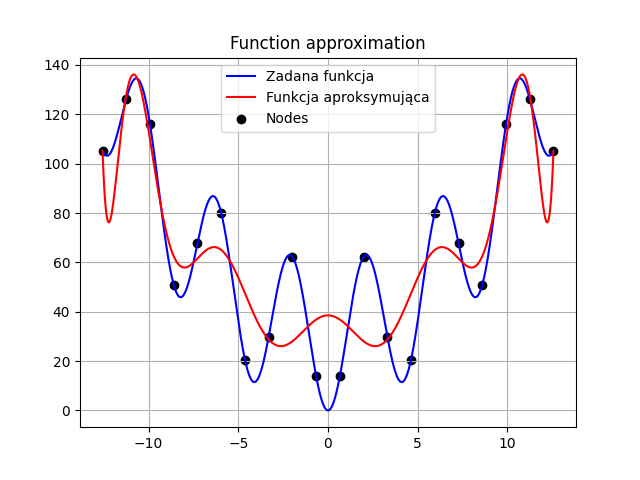
\includegraphics[width=\textwidth]{img19.png}
      \caption{Wielomian 12 stopnia}
    \end{minipage}
  \end{minipage}
\end{figure}

Poniżej, na wykresie 20 przedstawione zostały wartości błędów dla wszystkich możliwych stopni wielomianu.

\begin{figure}[H]
  \centering
  \begin{minipage}[b]{0.4\textwidth}
    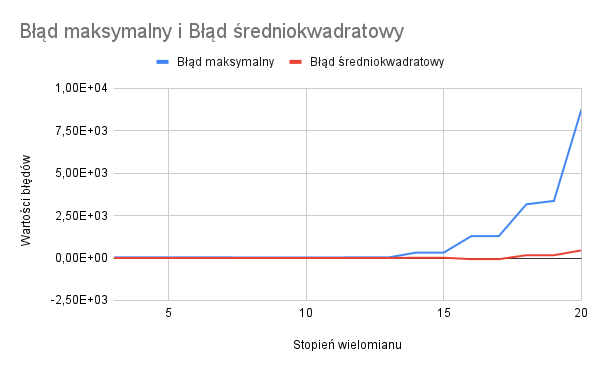
\includegraphics[width=\textwidth]{img20.png}
    \caption{Wartości błędów}
  \end{minipage}
\end{figure}

\newpage

\subsection{Dla 25 węzłów}

W tym przypadku otrzymałem jeszcze lepsze przybliżenie, natomiast nadal jest ono bardzo złe. Najlepszy okazał się wielomian stopnia 12, a potem błąd zaczął się bardzo szybko zwiększać (wykres 21, wykres 22, wykres 23 i wykres 24)

\begin{figure}[H]
  \begin{minipage}[b]{0.49\textwidth}
    \begin{minipage}[b]{\textwidth}
      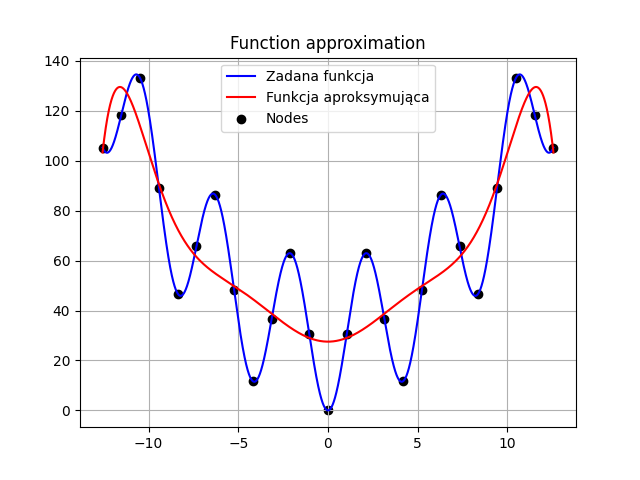
\includegraphics[width=\textwidth]{img21.png}
      \caption{Wielomian 11 stopnia}
    \end{minipage}
    \vspace*{\fill}
    \begin{minipage}[b]{\textwidth}
      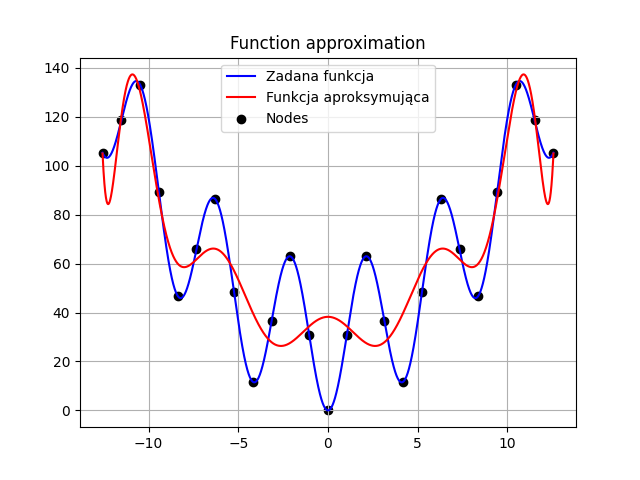
\includegraphics[width=\textwidth]{img22.png}
      \caption{Wielomian 12 stopnia}
    \end{minipage}
  \end{minipage}
  \hfill
  \begin{minipage}[b]{0.49\textwidth}
    \begin{minipage}[b]{\textwidth}
      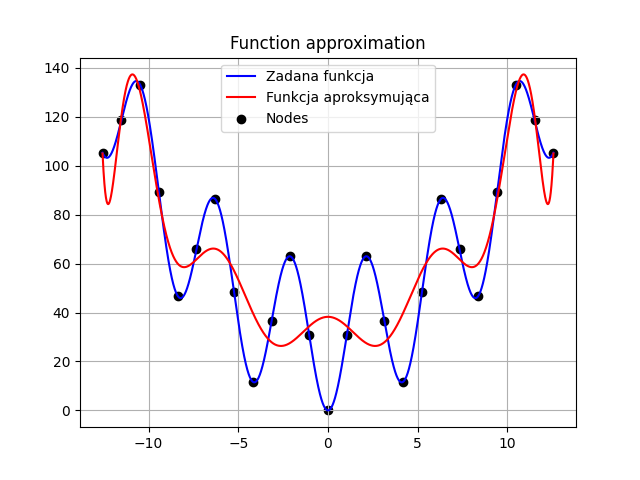
\includegraphics[width=\textwidth]{img23.png}
      \caption{Wielomian 13 stopnia}
    \end{minipage}
    \vspace*{\fill}
    \begin{minipage}[b]{\textwidth}
      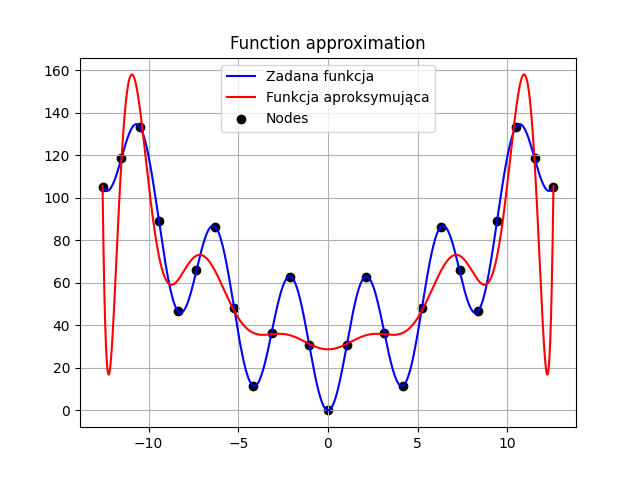
\includegraphics[width=\textwidth]{img24.png}
      \caption{Wielomian 14 stopnia}
    \end{minipage}
  \end{minipage}
\end{figure}

Poniżej, na wykresie 25 przedstawione zostały wartości błędów dla wszystkich możliwych stopni wielomianu.

\begin{figure}[H]
  \centering
  \begin{minipage}[b]{0.4\textwidth}
    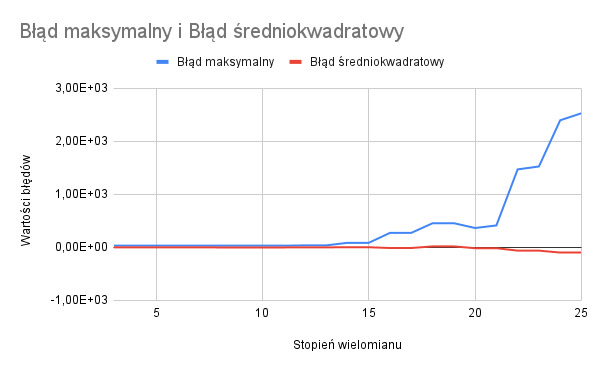
\includegraphics[width=\textwidth]{img25.png}
    \caption{Wartości błędów}
  \end{minipage}
\end{figure}

\newpage

\subsection{Dla 50 węzłów}

Dla 50 węzłów jesteśmy w stanie otrzymać lepsze przybliżenie, ale nadal za dobre przyblizenie w środku przedziału płacimy dużymi błedami na krańcach (wykres 26, wykres 27, wykres 28, wykres 29).

\begin{figure}[H]
  \begin{minipage}[b]{0.49\textwidth}
    \begin{minipage}[b]{\textwidth}
      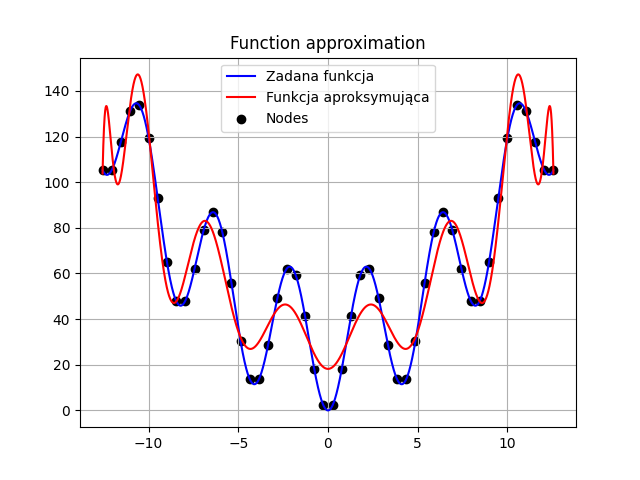
\includegraphics[width=\textwidth]{img26.png}
      \caption{Wielomian 17 stopnia}
    \end{minipage}
    \vspace*{\fill}
    \begin{minipage}[b]{\textwidth}
      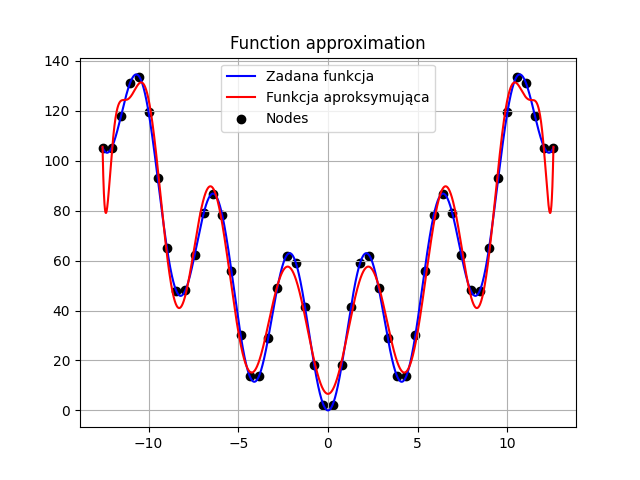
\includegraphics[width=\textwidth]{img27.png}
      \caption{Wielomian 18 stopnia}
    \end{minipage}
  \end{minipage}
  \hfill
  \begin{minipage}[b]{0.49\textwidth}
    \begin{minipage}[b]{\textwidth}
      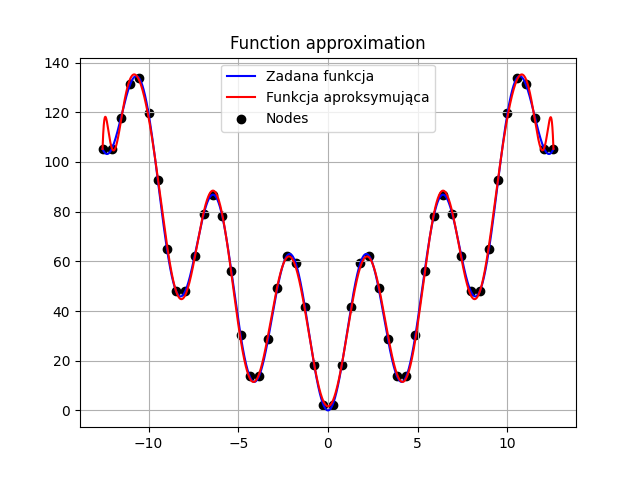
\includegraphics[width=\textwidth]{img28.png}
      \caption{Wielomian 21 stopnia}
    \end{minipage}
    \vspace*{\fill}
    \begin{minipage}[b]{\textwidth}
      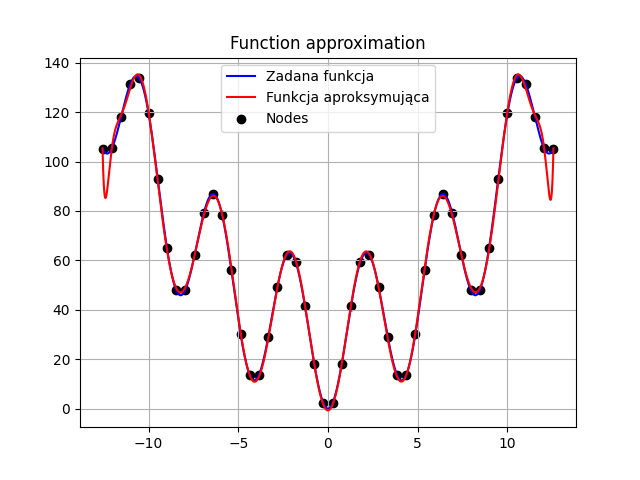
\includegraphics[width=\textwidth]{img29.png}
      \caption{Wielomian 22 stopnia}
    \end{minipage}
  \end{minipage}
\end{figure}

Poniżej, na wykresie 30 przedstawione zostały wartości błędów dla wszystkich możliwych stopni wielomianu.

\begin{figure}[H]
  \centering
  \begin{minipage}[b]{0.4\textwidth}
    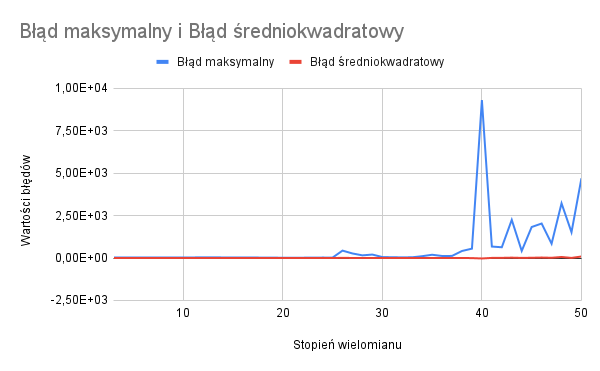
\includegraphics[width=\textwidth]{img30.png}
    \caption{Wartości błędów}
  \end{minipage}
\end{figure}

\newpage

\section{Przebieg funkcji dla wybranego stopnia wielomianu}

\subsection{Dla 6 stopnia}

Jak Widać, dla różnej liczby węzłów przebieg funkcji aproksymującej wygląda mniej więcej tak samo, z drobnymi różnicami na krańcach przedziałów (wykres 31, wykres 32, wykres 33, wykres 34)

\begin{figure}[H]
  \begin{minipage}[b]{0.49\textwidth}
    \begin{minipage}[b]{\textwidth}
      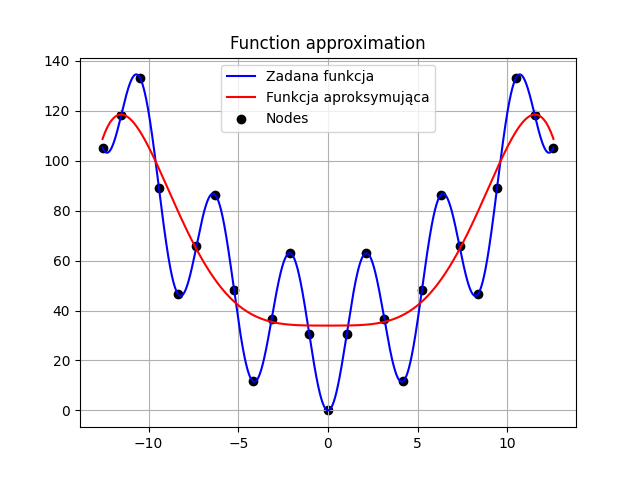
\includegraphics[width=\textwidth]{img31.png}
      \caption{Dla 25 węzłów}
    \end{minipage}
    \vspace*{\fill}
    \begin{minipage}[b]{\textwidth}
      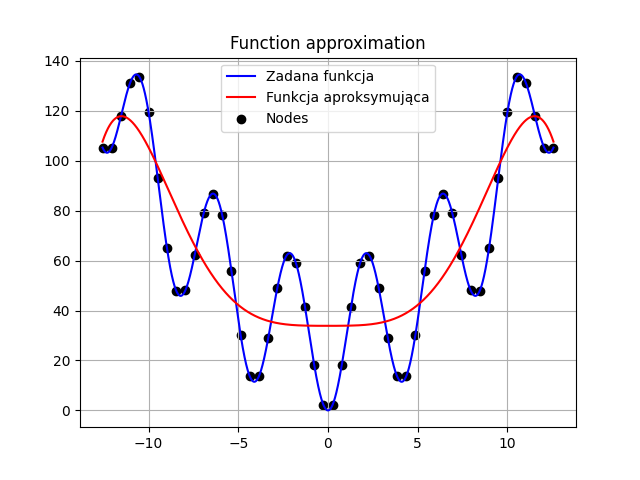
\includegraphics[width=\textwidth]{img32.png}
      \caption{Dla 50 węzłów}
    \end{minipage}
  \end{minipage}
  \hfill
  \begin{minipage}[b]{0.49\textwidth}
    \begin{minipage}[b]{\textwidth}
      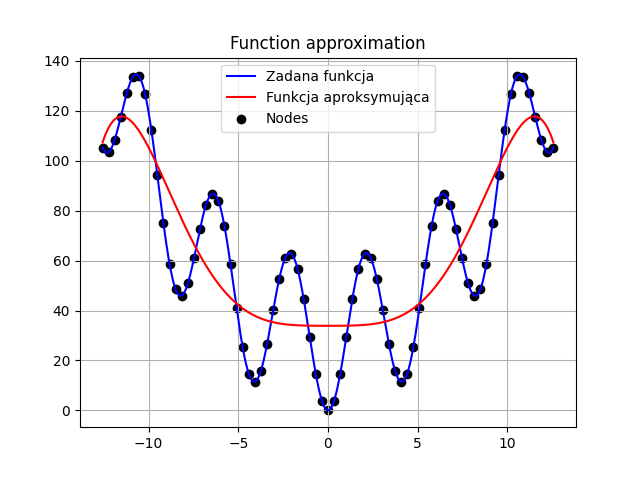
\includegraphics[width=\textwidth]{img33.png}
      \caption{Dla 75 węzłów}
    \end{minipage}
    \vspace*{\fill}
    \begin{minipage}[b]{\textwidth}
      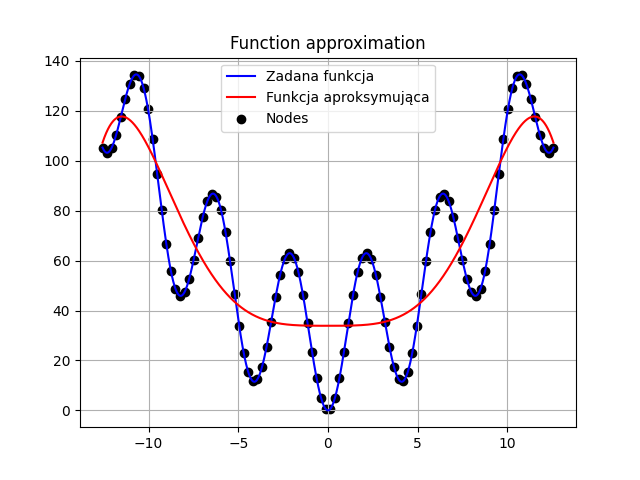
\includegraphics[width=\textwidth]{img34.png}
      \caption{Dla 100 węzłów}
    \end{minipage}
  \end{minipage}
\end{figure}

Poniżej, na wykresie 35 przedstawione zostały wartości błędów dla wszystkich możliwych stopni wielomianu.

\begin{figure}[H]
  \centering
  \begin{minipage}[b]{0.4\textwidth}
    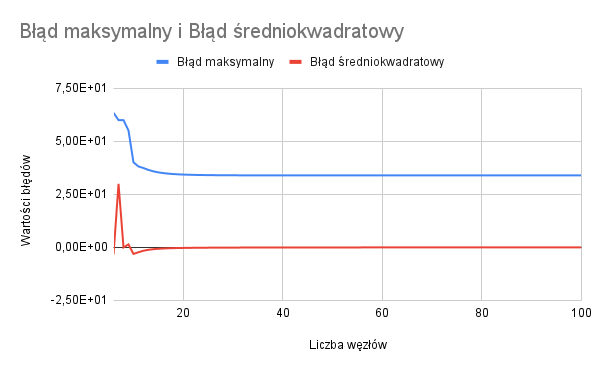
\includegraphics[width=\textwidth]{img35.png}
    \caption{Wartości błędów}
  \end{minipage}
\end{figure}

\subsection{Dla 10 stopnia}

Przybliżenie jest trochę lepsze na krańcach przedziału, jednak dalej funkcja aproksymująca przechodzi przez "środek" zadanej funkcji, co jest nieakceptowalne (wykres 36, wykres 37, wykres 38 i wykres 39).

\begin{figure}[H]
  \begin{minipage}[b]{0.49\textwidth}
    \begin{minipage}[b]{\textwidth}
      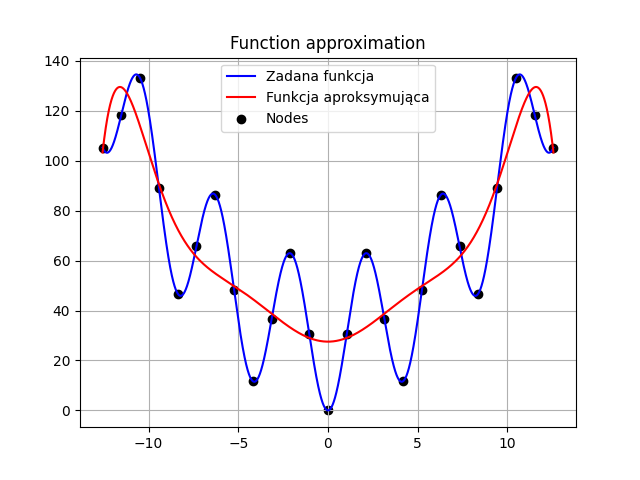
\includegraphics[width=\textwidth]{img36.png}
      \caption{Dla 25 węzłów}
    \end{minipage}
    \vspace*{\fill}
    \begin{minipage}[b]{\textwidth}
      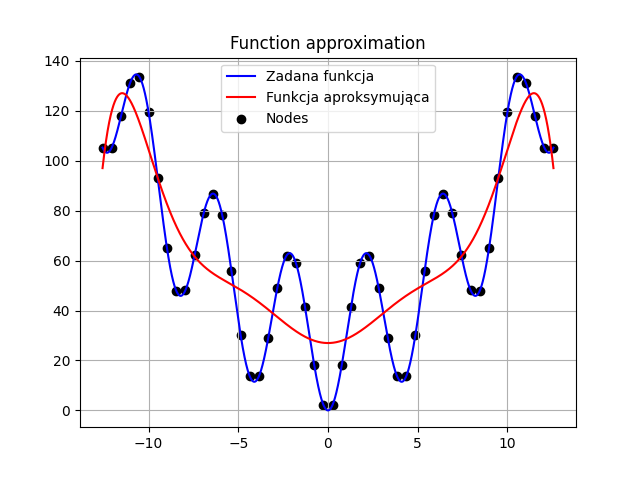
\includegraphics[width=\textwidth]{img37.png}
      \caption{Dla 50 węzłów}
    \end{minipage}
  \end{minipage}
  \hfill
  \begin{minipage}[b]{0.49\textwidth}
    \begin{minipage}[b]{\textwidth}
      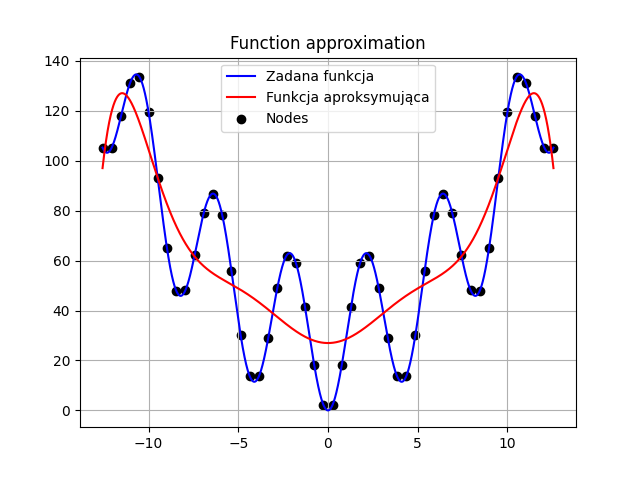
\includegraphics[width=\textwidth]{img38.png}
      \caption{Dla 75 węzłów}
    \end{minipage}
    \vspace*{\fill}
    \begin{minipage}[b]{\textwidth}
      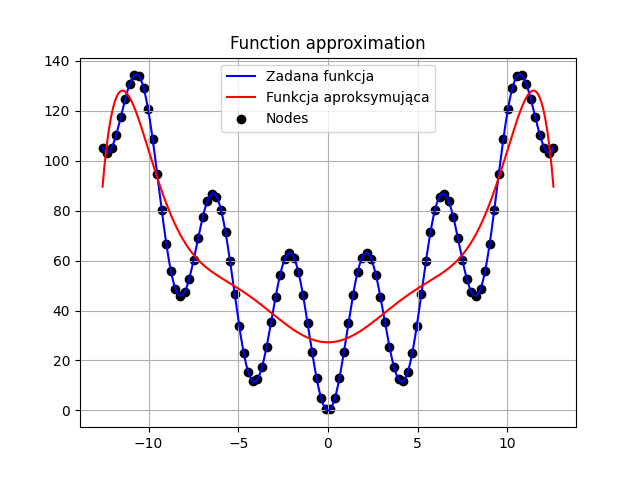
\includegraphics[width=\textwidth]{img39.png}
      \caption{Dla 100 węzłów}
    \end{minipage}
  \end{minipage}
\end{figure}

Poniżej, na wykresie 40 przedstawione zostały wartości błędów dla wszystkich możliwych stopni wielomianu.

\begin{figure}[H]
  \centering
  \begin{minipage}[b]{0.4\textwidth}
    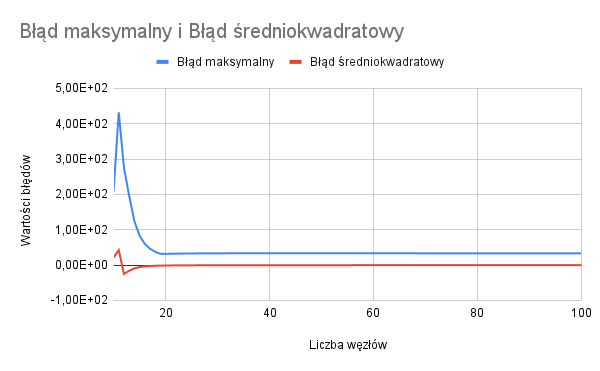
\includegraphics[width=\textwidth]{img40.png}
    \caption{Wartości błędów}
  \end{minipage}
\end{figure}

\newpage

\subsection{Dla 15 stopnia}

Jak widać na poniższych wykresach (wykres 41, wykres 42, wykres 43, wykres 44) dla 15 stopnia wielomianu otrzymujemy nieco lepsze przbliżenie, jednak dalej nie jest ono zadowalające.

\begin{figure}[H]
  \begin{minipage}[b]{0.49\textwidth}
    \begin{minipage}[b]{\textwidth}
      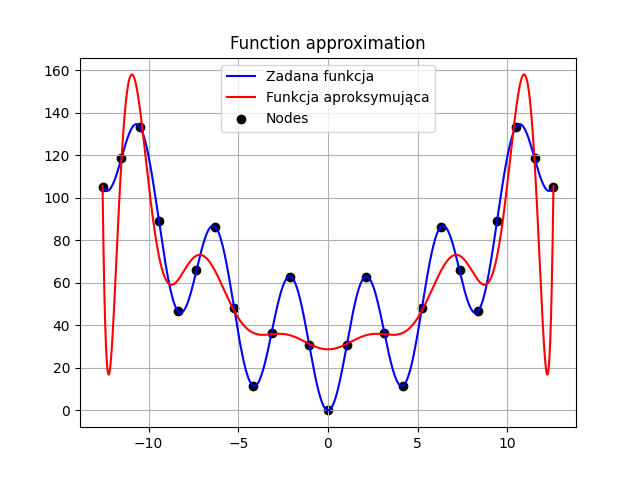
\includegraphics[width=\textwidth]{img41.png}
      \caption{Dla 25 węzłów}
    \end{minipage}
    \vspace*{\fill}
    \begin{minipage}[b]{\textwidth}
      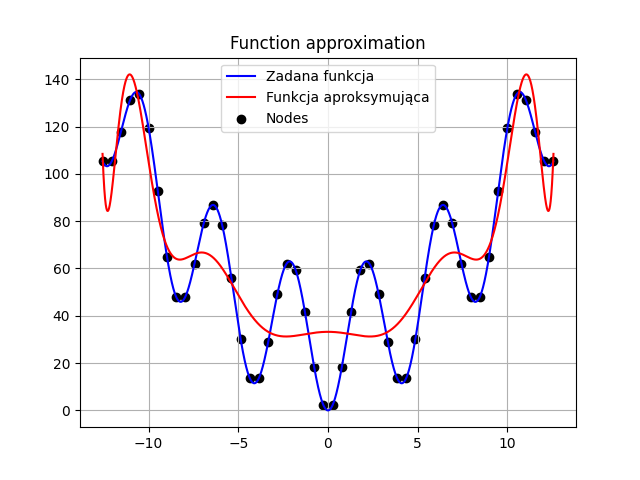
\includegraphics[width=\textwidth]{img42.png}
      \caption{Dla 50 węzłów}
    \end{minipage}
  \end{minipage}
  \hfill
  \begin{minipage}[b]{0.49\textwidth}
    \begin{minipage}[b]{\textwidth}
      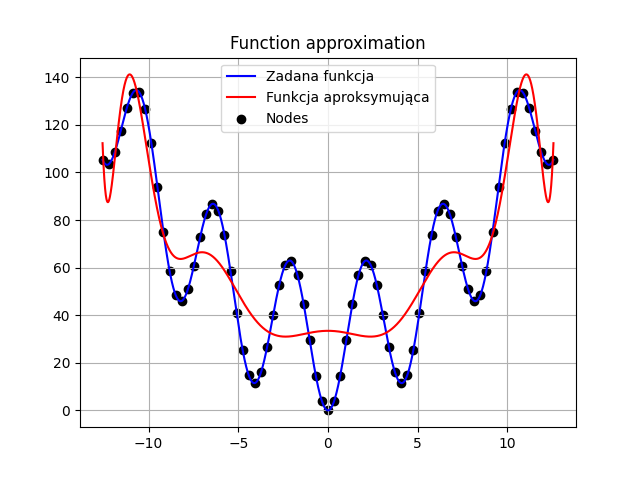
\includegraphics[width=\textwidth]{img43.png}
      \caption{Dla 75 węzłów}
    \end{minipage}
    \vspace*{\fill}
    \begin{minipage}[b]{\textwidth}
      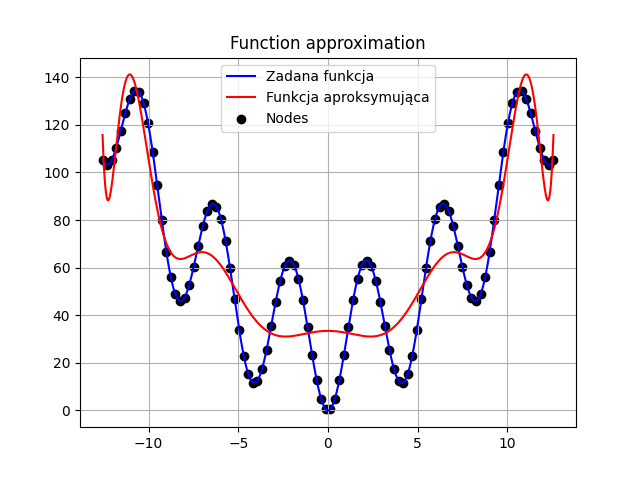
\includegraphics[width=\textwidth]{img44.png}
      \caption{Dla 100 węzłów}
    \end{minipage}
  \end{minipage}
\end{figure}

Poniżej, na wykresie 45 przedstawione zostały wartości błędów dla wszystkich możliwych stopni wielomianu.

\begin{figure}[H]
  \centering
  \begin{minipage}[b]{0.4\textwidth}
    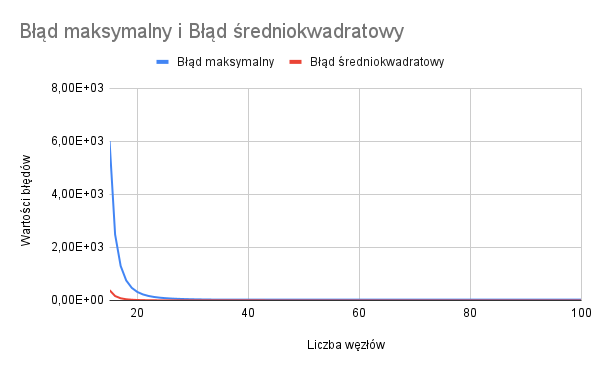
\includegraphics[width=\textwidth]{img45.png}
    \caption{Wartości błędów}
  \end{minipage}
\end{figure}

\newpage

\subsection{Dla 20 stopnia}

Dla 20 stopnia można już z pewnością powiedzieć, że przybliżenie jest dobre. Szczególnie jest to widoczne dla 100 węzłów, gdzie błędy na krańcach przedziałów są minimalne (wykres 46, wykres 47, wykres 48 i wykres 49).

\begin{figure}[H]
  \begin{minipage}[b]{0.49\textwidth}
    \begin{minipage}[b]{\textwidth}
      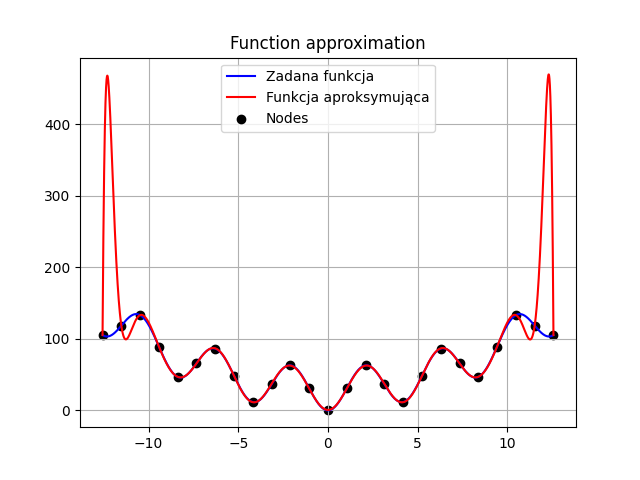
\includegraphics[width=\textwidth]{img46.png}
      \caption{Dla 25 węzłów}
    \end{minipage}
    \vspace*{\fill}
    \begin{minipage}[b]{\textwidth}
      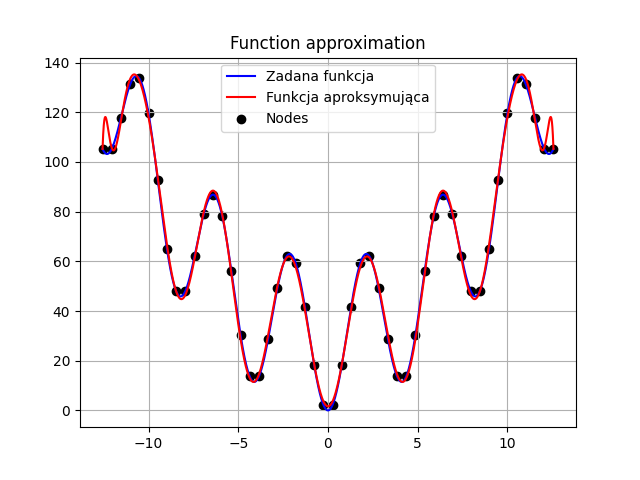
\includegraphics[width=\textwidth]{img47.png}
      \caption{Dla 50 węzłów}
    \end{minipage}
  \end{minipage}
  \hfill
  \begin{minipage}[b]{0.49\textwidth}
    \begin{minipage}[b]{\textwidth}
      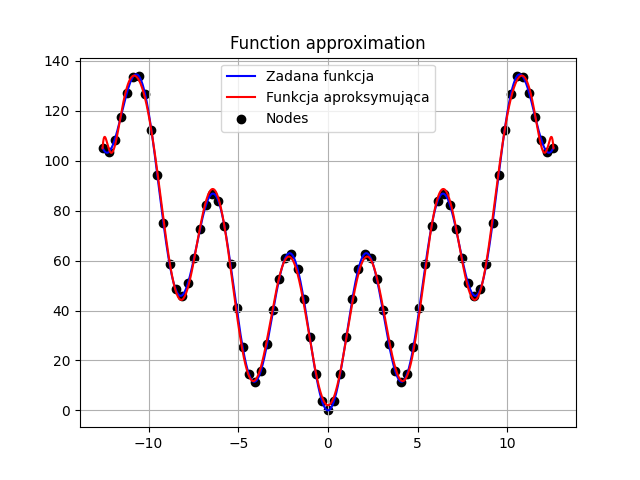
\includegraphics[width=\textwidth]{img48.png}
      \caption{Dla 75 węzłów}
    \end{minipage}
    \vspace*{\fill}
    \begin{minipage}[b]{\textwidth}
      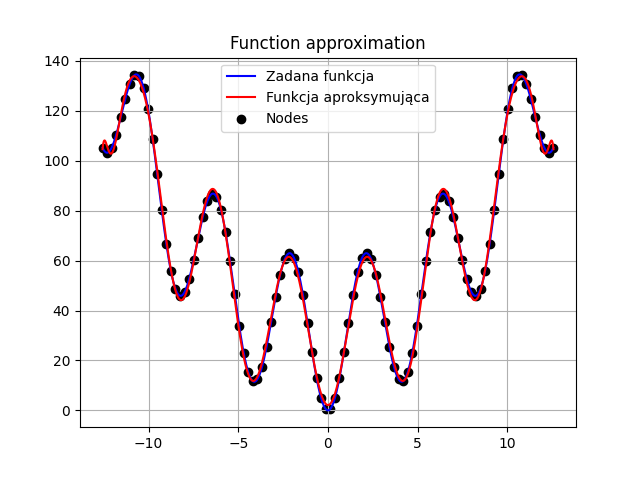
\includegraphics[width=\textwidth]{img49.png}
      \caption{Dla 100 węzłów}
    \end{minipage}
  \end{minipage}
\end{figure}

Poniżej, na wykresie 50 przedstawione zostały wartości błędów dla wszystkich możliwych stopni wielomianu.

\begin{figure}[H]
  \centering
  \begin{minipage}[b]{0.4\textwidth}
    \includegraphics[width=\textwidth]{img50.png}
    \caption{Wartości błędów}
  \end{minipage}
\end{figure}

\newpage

\subsection{Dla 25 stopnia}

Dla 25 stopnia wielomianu otrzymałem jeszcze lepsze przybliżenie, ponownie wraz z wzrostem liczby węzłów poprawia się przybliżenie, w szczegółności maleje błąd na krańcach przedziałów (wykres 51, wykres 52, wykres 53, wykres 54).

\begin{figure}[H]
  \begin{minipage}[b]{0.49\textwidth}
    \begin{minipage}[b]{\textwidth}
      \includegraphics[width=\textwidth]{img51.png}
      \caption{Dla 25 węzłów}
    \end{minipage}
    \vspace*{\fill}
    \begin{minipage}[b]{\textwidth}
      \includegraphics[width=\textwidth]{img52.png}
      \caption{Dla 50 węzłów}
    \end{minipage}
  \end{minipage}
  \hfill
  \begin{minipage}[b]{0.49\textwidth}
    \begin{minipage}[b]{\textwidth}
      \includegraphics[width=\textwidth]{img53.png}
      \caption{Dla 75 węzłów}
    \end{minipage}
    \vspace*{\fill}
    \begin{minipage}[b]{\textwidth}
      \includegraphics[width=\textwidth]{img54.png}
      \caption{Dla 100 węzłówa}
    \end{minipage}
  \end{minipage}
\end{figure}

Poniżej, na wykresie 55 przedstawione zostały wartości błędów dla wszystkich możliwych stopni wielomianu.

\begin{figure}[H]
  \centering
  \begin{minipage}[b]{0.4\textwidth}
    \includegraphics[width=\textwidth]{img55.png}
    \caption{Wartości błędów}
  \end{minipage}
\end{figure}

\newpage

\subsection{Dla 50 stopnia}

W tym przypadku nadal otrzymałem dobre przybliżenie, jednak z tego powodu, że stopień jest bliski liczbie węzłów występują duże błędy na krańcach przedziałów. Ponownie widać, że wraz z wzrostem liczby węzłów, rośnie dokładność (wykres 56, wykres 57, wykres 58, wykres 59).

\begin{figure}[H]
  \begin{minipage}[b]{0.49\textwidth}
    \begin{minipage}[b]{\textwidth}
      \includegraphics[width=\textwidth]{img56.png}
      \caption{Dla 50 węzłów}
    \end{minipage}
    \vspace*{\fill}
    \begin{minipage}[b]{\textwidth}
      \includegraphics[width=\textwidth]{img57.png}
      \caption{Dla 75 węzłów}
    \end{minipage}
  \end{minipage}
  \hfill
  \begin{minipage}[b]{0.49\textwidth}
    \begin{minipage}[b]{\textwidth}
      \includegraphics[width=\textwidth]{img58.png}
      \caption{Dla 90 węzłów}
    \end{minipage}
    \vspace*{\fill}
    \begin{minipage}[b]{\textwidth}
      \includegraphics[width=\textwidth]{img59.png}
      \caption{Dla 100 węzłówa}
    \end{minipage}
  \end{minipage}
\end{figure}

Poniżej, na wykresie 60 przedstawione zostały wartości błędów dla wszystkich możliwych stopni wielomianu.

\begin{figure}[H]
  \centering
  \begin{minipage}[b]{0.4\textwidth}
    \includegraphics[width=\textwidth]{img60.png}
    \caption{Wartości błędów}
  \end{minipage}
\end{figure}

\newpage

\section{Efekt Rungego}

Efekt Rungego mógł wystąpić, przy zbliżeniu sie do interpolacji, w moim przypadku największy błąd generował dla 40 węzłów i wielomianu 36 stopnia.

\begin{figure}[H]
  \centering
  \begin{minipage}[b]{0.4\textwidth}
    \includegraphics[width=\textwidth]{runge.png}
    \caption{Najlepsze przybliżenie funkcji}
  \end{minipage}
\end{figure}

\begin{table}[!ht]
    \centering
    \begin{tabular}{|l|l|}
    \hline
        Błąd maksymalny & 176413.32885002135    \\ \hline
        Błąd średniokwadratowy & 3832.7665755629732 \\ \hline
        
    \end{tabular}
\end{table}

\section{Najlepsze przyblizenie funkcji}

Najlepsze przybliżenie aproksymowanej funkcji otrzymałem dla 94 węzłów i wielomianu 25 stopnia, został on pokazany na poniższym wykresie, a jego błąd maksymalny i średniokwadratowy poniżej w tabelce. Można powiedzieć, że jest to naprawdę dobre przybliżenie.

\begin{figure}[H]
  \centering
  \begin{minipage}[b]{0.4\textwidth}
    \includegraphics[width=\textwidth]{best.png}
    \caption{Najlepsze przybliżenie funkcji}
  \end{minipage}
\end{figure}

\begin{table}[!ht]
    \centering
    \begin{tabular}{|l|l|}
    \hline
        Błąd maksymalny & 0.5014720569615605   \\ \hline
        Błąd średniokwadratowy & 0.0017181768299556364 \\ \hline
        
    \end{tabular}
\end{table}

\newpage

\section{Wnioski}

\begin{itemize}
\item Zwiększanie stopnia wielomianu dla ustalonej liczby węzłów powoduje zwiększejnie dokładności przybliżenia tylko do pewnego stopnia, potem zaczyna się zwiększać efekt Rungego i przybliżenie jest coraz gorsze
\item Zwiększanie liczby węzłów dla ustalonego stopnia wielomianu prowadzi do zwiększenia dokładności przyblizenia.
\item Wielomiany o dużym stopniu (30, 40, 50, ...) bardzo często stają się coraz mniej dokładne
\end{itemize}

\end{document}
